\section{Overview}
In order to pursue the goal of introducing contracts to BDD, three separate meta-models --- each with a specific purpose --– were created: One describing the BDD feature modeling language, one to model the transformation language and lastly, a model for describing a simplified version of JML.  Combined, they make it possible for contracts to be generated and extracted from feature descriptions and transformed into JML easing the continued work on a given software development project. Figure \ref{fig:overview} presents a brief overview of the workflow from input to output, i.e. how the different parts of the framework relate.

%%%
%%% Remember: Include floating for support of [h]-flag
%%%
\begin{figure}[h]
	\begin{center}
		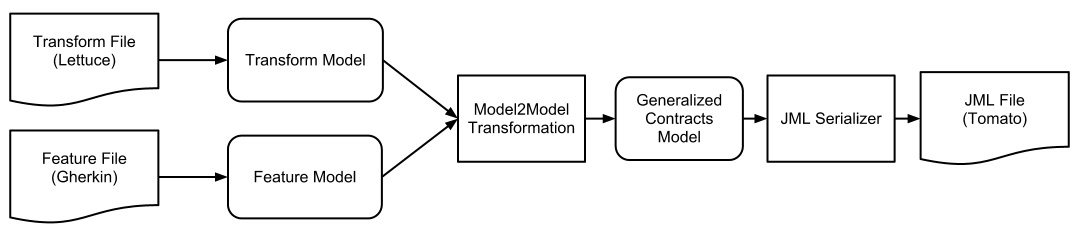
\includegraphics[scale=0.46]{images/framework_overview.png}
	\end{center}
	\caption{Salad Framework Workflow}
	\label{fig:overview}
\end{figure}

The feature meta-model represents an extension of BDD’s feature description which is the main artifact in BDD. By extending the original, well-known feature description language, instead of creating a new language, we allow people already familiar with BDD-features to work in an environment that they are accustomed to. The textual syntax of the new language parts introduced in this project is done with as much respect to the original language as possible. Having this rich model and language, that contains both the original features of the feature language as well as our extension, also allow for further development on the project as all elements of the language are available in the model. One could do a transformation to a simplified model accepted by standard BDD tools, which will allow the further generation of regular test-cases.

The transform model specifies how the contracts written in natural language in the feature file are transformed to actual contracts. By specifying rules on how contracts are interpreted the user decides the nature of the language in which the natural language contracts are represented. 

Through model-to-model transformation the feature model(s) and the transform model(s) are transformed into a meta-model representing a subset of JML, namely code contracts describing pre- and postconditions. The textual representation of our JML model resembles Java syntax with classes containing methods and their contracts written in JML.
